\documentclass[leqno,a4paper]{article}
\usepackage{hyperref}
\usepackage{caption}
\usepackage[T1]{fontenc}
\usepackage[utf8]{inputenc}
\usepackage{lmodern}
\usepackage[english]{babel}
\linespread{1.25} %easier reading/grading.
\usepackage{amsmath} %d'oh
\usepackage{amsfonts}
\usepackage{graphicx}
\usepackage{bold-extra} %for \mb
\usepackage[margin=2.5cm]{geometry} %for custom margins
\usepackage{enumerate} %for special counters
\usepackage{titlesec} %for section numbering
\usepackage{ifthen}
\renewcommand\thesubsection{\alph{subsection}}
\titleformat{\section}{\it \bf \large}{{\normalfont  \bf \thesection.}}{4pt}{}[]
\titleformat{\subsection}{\it \bf \large}{{\normalfont \bf \quad \large  \thesection \thesubsection)}}{5pt}{}[]
\titleformat{\subsubsection}{\bf \it}{\qquad}{5pt}{}[]

\numberwithin{equation}{section}
\newcommand\norm[1]{\left\lVert#1\right\rVert} %http://tex.stackexchange.com/questions/107186/how-to-write-norm-which-adjusts-its-size
\renewcommand{\O}{\mathcal{O}}
\renewcommand{\bf}{\bfseries}
\renewcommand{\sc}{\scshape}
\renewcommand{\it}{\itshape}
\renewcommand{\div}{\text{div }}
\renewcommand{\Re}{\mathbb{R}}
\newcommand{\op}{\left(}
\newcommand{\cp}{\right)}
\newcommand{\N}{\mathbb{N}}
\newcommand{\mb}{\mathbf}
\newcommand{\nn}{\\\nonumber}
\newcommand{\curl}{\text{curl }}
\renewcommand{\d}{\text{d}}
\newcommand{\inp}[2]{\left<#1, #2\right>}
\renewcommand{\d}[1]{\,\text{d}#1}
\newcommand{\pdrv}[2][x]{\frac{\partial #2}{\partial #1}}
\newcommand{\drv}[2][x]{\frac{\text{d} #2}{\text{d} #1}}
\renewcommand{\maketitle}[2][]{\begin{center}
{{\bf \huge \sc #2\\
\ifthenelse{\equal{#1}{}}{}{{\vspace{-12pt} \Large #1}\\\vspace{5pt}}
\begin{minipage}{1.0\textwidth}
  \raggedright
  {\large
   Roel Deckers}\\
   \normalsize
   roel@codingcat.nl\\
   930830-T150
\end{minipage}
\hfill
}}
\vspace{-1. cm}\rule[2.5 cm]{16 cm}{1 pt}
\vspace{-2.0 cm}
\end{center}}

\graphicspath{./plots}
\begin{document}
  \maketitle[High Performance Computing and Programming]{Exam Miniproject}

\section{Introduction}
I have split up the program in several different functions, and will discuss the optimizations applied to each part of the code in their own section.
\par These functions can be catagorized into: Allocations, allocating memory for all structures; Creating the random array of stars; Sorting the array; Filling the matrix with the right values
of starfunc and distances; Creating the values tallied in the histogram, that is the result of Neumann difference scheme on the matrix; and finally the creation of the histogram.
\par The project contains a single makefile which can build everything up to and including this report. Binaries are stored in the source folder and shared files in src/common.
the verify executable runs the supplied reference file. Verify\_large and verify\_large\_refference run the optimized and refference code on the same larger test case to verify that
the vector processing cases are handled correctlly. Timmings and timmings\_reference create timing data for various $N$ of each of the parts of the program for the optimized resp. refference
solution.
\par All tests were run on an AMD FX-8120 system running on a Windows system with gcc version 5.3.0 (Rev5, Built by MSYS2 project). The compiler flags used are
"-Ofast -flto -march=native".  An overview of the final speedup can be seen in figure \ref{fig:amd_fast} and figure \ref{fig:amd_slow}.
\par Performance was analyized using AMD's CodeXL profiler.

\begin{figure}[!Hhp]
  \centering
  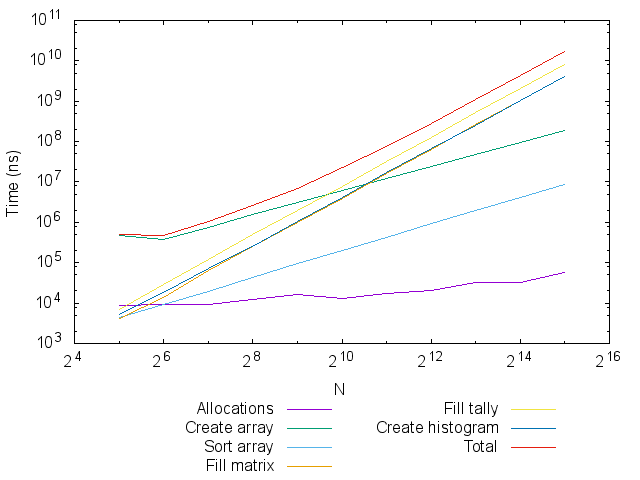
\includegraphics[width=\textwidth]{plots/timmings.png}
  \caption{Performance after optimization.}
  \label{fig:amd_fast}
  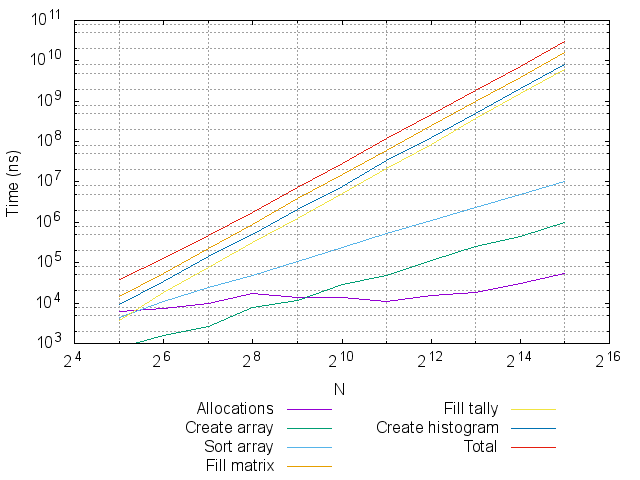
\includegraphics[width=\textwidth]{plots/timmings_reference.png}
  \caption{Performance before any optimizations}
  \label{fig:amd_slow}
\end{figure}

\section{Allocations}
This part of the code was not optimized as it is of approximately $\O(1)$ order and mostlly OS dependent. We could have slightlly optimized it by allocating a large buffer
in user-space and setting our own pointers in this space.

\section{Create Array}
This part of the code was modified to write a struct-of-arrays as opposed to an array-of-structs to allow for easier vectorization in the later parts and to not pollute cachelines
with unused variables such as 'designation'. For the random number generation we used a 32-bit LCG which provides us with very fast and repeatable random number generation. Whether this is a
realistic optimization depends on what one wishes to model and the requirements on the PRNG.

\section{Sorting}
For sorting the star array we used the quicksort algorithm.
because this was an $\O(n)$ process and the other functions were $\O(n^2)$ we have saved optimizing this function for last.
Unfortunately we were not able to fully optimize it due to time constraints,
however we have been able to improve the runtime by first computing the distances for each star and then storing this in a union with its index. Because distances are strictlly positive we can sort this union using
just integer arithmetic due to the way floating point numbers are stored. We then read this sorted list of indices and create a sorted array based on that information. This does slightlly increase memory usage, however only on the order of
$\O(n)$ whereas the global scaling is $\O(n^2)$. We tried to also vectorize the computation of the distances, however there is a bug in this particular implementation we have yet to track down and therefore it is commented out.
\par It might be possible to further improve performance by creating several bins corresponding to different distances and then storing the (distance, index) pairs in the corresponding bin as we are computing the distances.
This prefiltering should reduce the amount of iterations needed for the sorting algorithm to finish.

\section{Fill Matrix}
This is where the bulk of the speed was gained, compared to the original it is almost 10$\times$ faster, this is due to the 8 way vectorization and the linear-loads
 as a result of using a struct-of-arrays. There are virtually no cache-misses according to the profiler. One optimization which was tried but did not work was to use the much faster instruction for the
 reciprocal square root instead of the square root instruction. While this was much faster, the loss of accuracy led to NaN errors. It might be possible to further optimize this by using a different
 more accurate approximation for the root. We also rewrote the division in startfunc to be a multiplication and expressed it in such a way that it is clear to the compiler that we are performing a series of
 fused-multiply-add instructions.
 \par We also saved a large amount of memory here, (and run-time) by noting that the matrix is symmetric we only have to store half of the points. We in fact store slightly more because we store this matrix in a block upper-diagonal matrix with
 a blocksize of $8\times8$ to help with vectorization.

 \section{Fill tally}
 \par This function was the hardest to optimize, most notably due to vectorization and the fact that we store our previous matrix in block diagonal form. Nevertheless we got a
 significant speedup. Notablly by vectorization and by noting that the contibutions between neighbouting points are symmetric and therefore we only have to compute them once for each pair instead of for
 each point. Several attempts (on paper) were made to efficientlly vectorize this code, possibly by changing the data structure, but in the end I chose to apply a simple scheme which uses unalligned loads to line up
 the correct vector-lanes. According the AMD's CodeXL this instruction is now ~75\% of the runtime of the function, this is because unaligned loads are rather expensive on this particular CPU, but nevertheless performance was increased by adding vectorization.
 (and on later Intel CPUs the penalty for misaligned loads is minimal so perfomance gains will be even better there).
 \par Here too, the resulting matrix is symmetrical and so we store it as a tridiagonal matrix (as a flat array). When computing the histogram we take care to only count the diagonal elements once
 but the other elements twice.
 \par For added perfomance increase we could compute the min and max in this loop and pass that to the histogram algorithm, this gave a Performance boost before but was removed when I started to vectorize the code and has not yet been
 added back.

\section{Create Histogram}
Not much optimization was applied to this function yet, any speedup is due to the reduction of the size of the tally-matrix and by directlly computing the
index of an element instead of using a loop. I tried to replace the division by a multiplication, but there was no measurable difference. We could vectorize the index
computation, but to the best of my knowledge there is no way to use the resulting indices directlly in vector operations afterwards on the development machine.

\end{document}
